\chapter{Aufbau}
Zur Umsetzung des Deferred-Shadings wurde OpenGL als Grafikschnittstelle verwendet. Die nötige Kontext-Erstellung und das laden der OpenGL-Extensions wurden SDL und GLEW genutzt. Nach der Erstellung eines Fensters und der Initialisierung von OpenGL, werden zunächst alle benötigten Resource, wie etwa die verwendeten Shader, Texturen und Modelle geladen. Außerdem wird der G-Buffer mithilfe eines Framebuffer angelegt. Diesem werden vier Texturen, den sog. Framebuffer-Attachments, zur Speicherung der verschiedenen Informationen die für den Shading-Vorgang benötigt werden, hinzugefügt. In das erste Attachment wird der Depth-Buffer gerendert. Die übrigen drei Attachments beinhalten die Albdeo-Color, Normalen in Weltkoordinaten und den Spekular-Koeffizienten.

Das Layout des G-Buffers ist in \ref{fig:gbuffer} abgebildet.

\begin{figure}
\center
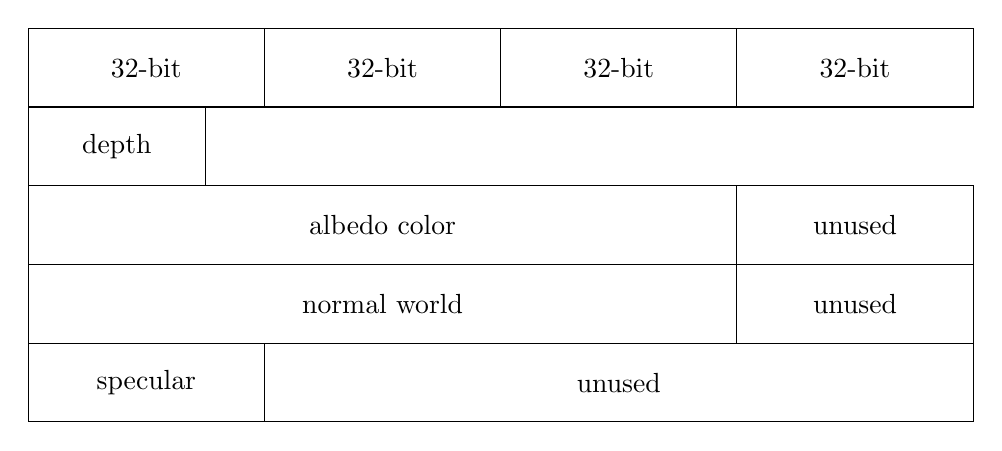
\begin{tikzpicture}
\draw (0,0) rectangle (3,-1) node[pos=.5]{32-bit};
\draw (3,0) rectangle (6,-1) node[pos=.5]{32-bit};
\draw (6,0) rectangle (9,-1) node[pos=.5]{32-bit};
\draw (9,0) rectangle (12,-1) node[pos=.5]{32-bit};
\draw (0,-1) rectangle (2.25,-2) node[pos=.5]{depth};
\draw (0,-2) rectangle (9,-3) node[pos=.5]{albedo color};
\draw (9,-2) rectangle (12,-3) node[pos=.5]{unused};
\draw (0,-3) rectangle (9,-4) node[pos=.5]{normal world};
\draw (9,-3) rectangle (12,-4) node[pos=.5]{unused};
\draw (0,-4) rectangle (3,-5) node[pos=.5]{specular};
\draw (3,-4) rectangle (12,-5) node[pos=.5]{unused};
\end{tikzpicture}
\caption{G-Buffer Layout}
\label{fig:gbuffer}
\end{figure}

In der Renderfunktion wird die Szenen-Geometrie nun gerendert und im Fragment-Shader die einzelnen Komponenten des G-Buffers befüllt. Lediglich der Depth-Buffer muss nicht selbst befüllt werden, da Framebuffer in OpenGL nur ein Depth-Attachment haben können und dieses als Depth-Buffer verwendet wird, sobald der Framebuffer gebunden wurde. Nach dem füllen des G-Buffers wird der Kompositionsschritt durchgeführt, mit dem das finale Bild berechnet wird. Hierzu wird ein Rechteck mit der Größe des Fensters gerendert und anschließend im Fragment-Shader die Beleuchtung berechnet. In diesen werden neben der Position, Farbe und dem Radius des Lichtes auch noch die einzelnen Attachments des G-Buffers und die Inverse View-Projection-Matrix übergeben. Diese wird benötigt um die frühere Position des Fragments in Weltkoordinaten zu ermitteln.

Dazu wird zunächst der Tiefenwert an der Stelle aus dem Depth-Attachment gelesen, die relativ zur Position des Fragments auf dem Bildschirm liegt. Dieser Wert liegt im Bereich [0,1], wobei 0 die Near-Plane ist und 1 die Far-Plane. Um die Z-Position in Weltkoordinaten zu erhalten muss der Tiefenwert in den Wertebereich [-1,1] gebracht werden.
Anschließend werden Fragmentposition und Tiefenwert in einem 4-Komponenten-Vektor zusammengefasst und die inverse View-Projection-Matrix mit diesem multipliziert. Der daraus resultierende Vektor wird durch seine vierte Komponente geteilt um die Position des Fragments in Weltkoordinaten zu erhalten. Nun kann die Berechnung der Beleuchtung erfolgen.

Für die Berechnung der Beleuchtung wurde das Modell von Blinn verwendet. Die verwendeten Lichtquellen sind ausschließlich Punkt-Lichtquellen. Außerdem wurde Tangent-Space-Normalmapping verwendet.